\documentclass[twoside, openright, 12pt]{book}
\sloppy

% Preamble
% General Setup
\usepackage{ifthen}		% If-Then-Statements
\usepackage{pdfpages}
\usepackage{hyperref}		% Hyperlinks & PDF specific information
\hypersetup{
	pdftitle={Master thesis - Philipp Schwetschenau},
	pdfsubject={Master thesis},
	pdfauthor={Philipp Schwetschenau},
	pdfborder={0 0 0}
}
\usepackage[nounderscore]{syntax}

% Language & Encoding
\usepackage[T1]{fontenc}
\usepackage[USenglish]{babel}
\usepackage[fixlanguage]{babelbib}
\usepackage[utf8]{inputenc}
\usepackage{blindtext}
\usepackage{caption}

% Page Geometry
\usepackage[a4paper]{geometry}
\geometry{
	twoside,
	top=3cm,
	bottom=3cm
}

% Literature
\usepackage{url}
\usepackage[sort&compress,square,comma,authoryear]{natbib}

% Fonts & Symbols
\usepackage{latexsym}		% Rare symbols
\usepackage{amsfonts}		% Math fonts
\usepackage{amssymb}		% Symbols
\usepackage{amsmath}		% Symbols
\usepackage{lmodern}		% "Latin Modern" ("Computer Modern"++)

\newcommand{\origttfamily}{}	% Separator for typewriter
\let\origttfamily=\ttfamily
\renewcommand{\ttfamily}{\origttfamily \hyphenchar\font=`\-}


%
% Document Layout

\usepackage[activate]{pdfcprot}	% margin kerning

% Header & Footer
\usepackage{fancyhdr}		% format headers
\pagestyle{fancy}
\fancyhf{}
\setlength{\headheight}{15pt}
\fancyhead[LE,RO]{\sffamily \thepage}
\fancyhead[RE]{\sffamily \nouppercase{\leftmark}}
\fancyhead[LO]{\sffamily \nouppercase{\rightmark}}
\renewcommand{\headrulewidth}{0.4pt}
\fancypagestyle{plain}{
	\fancyhead[RE,LO]{}
	\renewcommand{\headrulewidth}{0pt}
}
\fancypagestyle{simple}{
	\fancyhead[RE,LO]{}
	\renewcommand{\headrulewidth}{0pt}
}
\fancypagestyle{light}{
	\fancyhead[RE,LO]{}
}

% ClearDoublePage fix
\makeatletter 
\def\cleardoublepage{\clearpage\if@twoside \ifodd\c@page\else% 
\hbox{}% 
\thispagestyle{simple}
\newpage% 
\if@twocolumn\hbox{}\newpage\fi\fi\fi}
\makeatother 

% Headlines
\usepackage{titlesec}
\setcounter{secnumdepth}{3}
\titleformat{\chapter}[display]%
	{\huge\center\bf}%
	{\large\mdseries CHAPTER \thechapter}%
	{0cm}{}[\vspace{2ex}\titlerule]
\titlespacing*{\chapter}{0pt}{0ex}{8ex}
\titleformat{\subsubsection}{\normalsize\bfseries}{\thesubsubsection}{.75em}{}
\titleformat{\paragraph}[runin]{\bfseries}{}{0pt}{}[.]
\titleformat{\subparagraph}[runin]{\itshape}{}{0pt}{}[.]

% Table of Contents
\usepackage[titles]{tocloft}

\setlength{\cftbeforetoctitleskip}{0ex}
\setlength{\cftaftertoctitleskip}{0ex}
\renewcommand{\cfttoctitlefont}{}

\setlength{\cftbeforeloftitleskip}{4ex}
\setlength{\cftafterloftitleskip}{1ex}
\renewcommand{\cftloftitlefont}{\LARGE}

\setlength{\cftbeforelottitleskip}{4ex}
\setlength{\cftafterlottitleskip}{1ex}
\renewcommand{\cftlottitlefont}{\LARGE}

\newcommand\listingname{Verzeichnis der Listings}
\newlistof[chapter]{listing}{lst}{\listingname}
\setlength{\cftbeforelsttitleskip}{4ex}
\setlength{\cftafterlsttitleskip}{1ex}
\renewcommand{\cftlsttitlefont}{\LARGE}

\newcommand\theoremsname{Theoremverzeichnis}
\newlistof[chapter]{theorems}{lthm}{\theoremsname}
\setlength{\cftbeforelthmtitleskip}{4ex}
\setlength{\cftafterlthmtitleskip}{1ex}
\renewcommand{\cftlthmtitlefont}{\LARGE}

\setcounter{tocdepth}{2}
\setlength{\cftbeforechapskip}{1.0ex}
\setlength{\cftbeforesecskip}{0ex}
\setlength{\cftbeforesubsecskip}{-.2ex}
\newcommand\tocentry[1]{\addcontentsline{toc}{chapter}{#1}}
\newcommand{\ttsubsection}[1]{\subsection[\texorpdfstring{\texttt{\slshape #1}}{#1}]{\texttt{#1}}}
\newcommand\addtotheorems[2]{
	\refstepcounter{theorems}
	\addcontentsline{lthm}{theorems}{\protect\numberline{\thetheorems}\textbf{#1:} #2}
}
\newcommand\addlistspace[1]{
	\addtocontents{#1}{\vspace{1.3ex}}
}

% Glossar
\usepackage[number=none,style=altlist]{glossary}
\renewcommand{\glosslabel}[2]{\sffamily #2}
\makeglossary


%
% Page Elements

% Captions & Figures
\usepackage{graphicx}		% include graphics
\graphicspath{{./figures/}}

% Tables
\usepackage{booktabs}

% Theorems
\usepackage{framed}		% Frames for theorems.
\usepackage[framed,thmmarks,amsmath]{ntheorem}	% extended theorem enviroments
\usepackage{shadethm}		% theorems with colored background
\theoremheaderfont{\sffamily\bfseries}
\theorembodyfont{}
\theoremstyle{break}
\theoremseparator{.}
\theoremindent0cm
\theoremsymbol{}

\newshadetheorem{xtheorem}{Theorem}[chapter]
\newshadetheorem{xlemma}[xtheorem]{Lemma}
\newshadetheorem{xdefinition}[xtheorem]{Definition}
\newshadetheorem{xrequirement}[xtheorem]{Requirement}

\newenvironment{theorem}[1][]{%
	\addtotheorems{Theorem}{#1}
	\begin{xtheorem}[#1]%
}{\end{xtheorem}}
\newenvironment{lemma}[1][]{%
	\addtotheorems{Lemma}{#1}
	\begin{xlemma}[#1]%
}{\end{xlemma}}
\newenvironment{definition}[1][]{%
	\addtotheorems{Definition}{#1}
	\begin{xdefinition}[#1]%
}{\end{xdefinition}}
\newenvironment{requirement}[1][]{%
	\addtotheorems{Requirement}{#1}
	\begin{xrequirement}[#1]%
}{\end{xrequirement}}

\newshadetheorem{xapxtheorem}{Theorem}[section]
\newenvironment{apxtheorem}[1][]{%
	\addtotheorems{Theorem}{#1}
	\begin{xapxtheorem}[#1]%
}{\end{xapxtheorem}}

\theoremstyle{nonumberplain}
\theoremseparator{.}
\theoremheaderfont{\sffamily\itshape}
\theoremsymbol{\ensuremath{\Box}}
\newtheorem{proof}{Proof}
\newtheorem{apxproof}{Proof}

% Listings
\usepackage{listings}
\lstset{
	basewidth={0.5em,0.45em},
	frame=lines,
	framerule=\lightrulewidth,
	captionpos=b,
	lineskip=-1pt,
%	float=hbt,
	xleftmargin=1cm,
	xrightmargin=1cm,
	aboveskip=0.5cm,
	belowskip=0.5cm,
}
\lstnewenvironment{java}[2]{
	\refstepcounter{listing}
	\addcontentsline{lst}{listing}{\protect\numberline{\thelisting}#1}
	\lstset{
		language=C++,
		basicstyle=\ttfamily,
		commentstyle=\sffamily,
		lineskip=-2pt,
		tabsize=4,
		#2
	}
}{}
\lstdefinelanguage{pseudocode}{
	sensitive=true,
	alsodigit={:},
	morekeywords={
		Algorithmus,Eingabe:,Ausgabe:,Variablen:,%
		when,if,then,else,end,atomic,out,%
		case,is,repeat,while,do,until},
}
\lstdefinelanguage[distributed]{pseudocode}
	[]{pseudocode}{
	alsodigit={:},
	morekeywords={Async,Sync,%
		Constants:,Variables:,Input:,Action:,Action,%
		send,to,from},
	deletekeywords={Algorithmus,Eingabe:,Ausgabe:,Variablen:}
}
\newcommand{\setpseudocode}[2]{
	\lstset{
		% Syntax
		language=[#1]{pseudocode},
		mathescape=true,
		escapechar=\#,
		tabsize=4,
%		gobble=4,
		literate={:=}{{$\gets$}{\:}}2 {->}{{$\rightarrow$}{\:}}2,
		% Style
		basicstyle=\rmfamily,
		commentstyle=\sffamily,
		moredelim=[is][\itshape]{//}{//},
		moredelim=[il][\sffamily]{**},
		% Layout & Placement
		numbers=left,
		numberstyle=\tiny,
		columns=flexible,
		breaklines=true,
		breakatwhitespace=true,
		breakindent=2em,
		% User defined
		#2
	}
}
\lstnewenvironment{distalg}[2]{%
	\refstepcounter{listing}
	\addcontentsline{lst}{listing}{\protect\numberline{\thelisting}#1}
	\setpseudocode{distributed}{#2}
}{}
\lstnewenvironment{pseudocode}[2]{%
	\refstepcounter{listing}
	\addcontentsline{lst}{listing}{\protect\numberline{\thelisting}#1}
	\setpseudocode{}{#2}
}{}

\newcommand\textcall[1]{\textsc{#1}}
\newcommand\call[2]{\ensuremath{\operatorname{\textcall{#1}}(#2)}}
\newcommand\callname[2]{\ensuremath{\operatorname{#1}(#2)}}
\newcommand\topin[1]{\ensuremath{\operatorname{In}({#1})}}
\newcommand\topout[1]{\ensuremath{\operatorname{Out}({#1})}}


%
% Inline
\usepackage{url}		% Cite URLs
\usepackage{numprint}		% Format numbers
\newcommand\notice[1]{}		% Notice
\newcommand\seppar{ \vspace{2ex} \noindent } % New paragraph
\newcommand\name[1]{{\em #1}} 	% Names


\newenvironment{BNF}
  {\captionsetup{type=lstlisting}}
  {}

\begin{document}

%
% Titelseite
\begin{titlepage}
\newlength{\detailwidth}
\newlength{\detaildescriptionwidth}
\settowidth{\detailwidth}{Eingereicht:~~ Prof. Dr.-Ing. habil. Winfried E. Kühnhauser}
\settowidth{\detaildescriptionwidth}{Studies:~~} 
\begin{center}

\vfill {
	
\includegraphics[width=6cm]{logo-tu-ilmenau.jpg}
	\vspace{8ex}
}

\begin{normalsize}Technische Universität Ilmenau \\
Fakultät für Informatik und Automatisierung \\
Institut für Praktische Informatik und Medieninformatik \\
Fachgebiet für Verteilte Systeme und Betriebssysteme        
\end{normalsize}


\vfill {\large
	Masters thesis\\ \vspace{2ex}
	\LARGE \textbf{Graphical Specification Language for the Entity-Labeling Aspect} \\ \vspace{2.5ex} 
	\normalsize Submitted by: \\
	\Large Philipp Schwetschenau \\ \vspace{3ex} 
}
\vfill \parbox{\detailwidth}{
	\makebox[\detaildescriptionwidth][r]{Supervisor:~~} Prof. Dr.-Ing. habil. Winfried E. Kühnhauser \\
	\makebox[\detaildescriptionwidth][r]{Supervisor:~~} Dipl.-Inf. Peter Amthor \\
	\vspace{2ex} \\
	\makebox[\detaildescriptionwidth][r]{Studies:~~} Computer science\\  
	\makebox[\detaildescriptionwidth][r]{Matriculation no.:~~} 46756  
	\vspace{2ex} \\
	\makebox[\detaildescriptionwidth][r]{Submission date:~~} Ilmenau, 29. November 2018 
}
\vspace*{\fill}
\end{center}
\end{titlepage}

\mbox{}
\thispagestyle{empty}
\cleardoublepage

% Gliederung
\pagenumbering{roman}
\setcounter{page}{1}
\tableofcontents

% Abbildungsverzeichnis
\cleardoublepage
\listoffigures
\tocentry{List of figures}

%\listoflisting
%\tocentry{\listingname}

%
% Citing

% Author 1 et al. [1234]
%\cite{Harrison75a}

% Author 1, Author 2, Author 3 [1234]
%\cite*{Harrison75a}

% [Author 1 et al. 1234]
%\citep{Harrison75a}

% [Author 1, Author 2, Author 3 1234]
%\citep*{Harrison75a}



% Inhalts-Teil
\cleardoublepage
\pagenumbering{arabic}
\chapter{Introduction}
\label{introduction}

\section{Domain} 
\label{domain}
With the increasing number of IT systems, securing these systems became an obvious and important issue.
For this purpose many security models and model families were developed for a wide field of application domains over the last years.

Formal security models offer possibilities to analyze them concerning security properties.
However, because quantity and variety of these models grow just as much as their relevance for security-critical applications the model-based security engineering process became more complex and therefore error-prone to human deviations.

\citet*{Amthor18} proposed a new approach called Aspect-oriented Security Engineering (AOSE) which claims to close semantic gaps between steps in the security engineering process (requirements, informal policy, formal model) to reduce the potential impact of human errors.
This approach roughly adopts the idea of the aspect-oriented programming paradigm.
It tailors all steps to aspects, which are non-functional requirements of the engineering process like determining requirements of policy semantics or analyzing certain security goals.
There are two major classes for aspects regarding AOSE: related to policy semantics and to policy analysis.

One possible aspect of the former is the Entity Labeling Aspect (EL).
It is designed to formally specify policy semantics typically found in operating systems and middleware systems.
Therefore it bridges the gap and supports the transformation between informal policy and formal model.
EL classifies model components into six semantic categories.
The notation is on a mathematical basis and uses concepts like sets, assignments or constraints.



\section{Motivation} 
\label{motivation}
The goal of reducing the impact of human errors by closing semantic gaps as much as possible with the help of AOSE/EL requires handling another formal notation, which is, in this case, EL itself and its classification into the six semantic categories.
To support working with this approach, especially for the communication between different groups of people involved like model engineers, security architects, software developers or future administrators, who have to cooperate and coordinate and all have different levels of experience, \citet*{Amthor18} considers a graphical representation to be helpful to enhance the transition between informal and formalized notation.

\citet*{Amthor18} already uses visual representations to illustrate examples.
However, the representations are not described in detail as well as they are inconsistent and ambiguous regarding several parts of the formalization (e.g.\ arrows can have several meanings and there is no way to specify functions with multiple input parameters).
So these visualizations are appropriate to underline and support the engineering of an already formalized policy after EL-based model engineering, but are not suitable for independent modeling on a stand-alone level, because they are not equivalent to their formalized mathematical counterpart.

There are two types of visualization \cite{Amthor18} uses, which have different levels of abstraction: 
One is based on the actual model components and visualizes them and their relationships.
The other one is based on a higher level of abstraction and visualizes the EL with its structure of semantic categories and their relationships.

There are other visual notations like UML or ERD, which have in common that they are tailored to particular needs in special application domains, so they can not be applied here, but may give inspiration on how to model certain semantics and relationships.

Eventually to be able to independently and visually model and work on EL-based policies there is need for an unambiguous formal graphical specification language.



\section{Goal}
\label{goal}
The main goal is to develop a graphical specification language for EL-based security polices.
This should focus on clean and unambiguous semantics of the language.

The use of the language should be as simple as possible and as comprehensive as needed.
Therefore its appearance and elements should be clear and well-structured.
A selection of appropriate symbols and geometrical shapes for their equivalent model counterparts has to be made regarding an intuitive understanding and workflow.
This selection should not be designed contradictory or conflicting to already established notations, especially those, which may be used in the context of security engineering.

It should be evaluated how feasible and reasonable it is to develop equivalent counterparts for every possible element and relationship in context of EL and to display all of them at once.
This may also lead to the question how the visualization is related to a visualization on a higher abstraction level and how they are connected and might be managed.
The latter may be investigated as an optional goal.

In addition to that a GUI-based editor should be developed as a prototype to make use of the proposed graphical specification language.



\section{Structure}
\label{structure}




\cleardoublepage
\chapter{Fundamentals}
\label{fundamentals}
This chapter provides information to all fundamentals necessary for this thesis.
It will serve as basis for all design decisions in the following chapter~\ref{gsl_design} and chapter~\ref{editor_design}.

Section \ref{security_models} introduces the RBAC security model.
Section \ref{AOSEEL} focuses on the Aspect-oriented Security Engineering (AOSE) proposed by \citet*{Amthor18}.
It covers the Entity-Labeling Aspect in particular, one aspect of AOSE, which is going to be essential regarding the task to design a graphical specification language for it in chapter~\ref{gsl_design}.
In section~\ref{graphical_notations} the well-established graphical notations UML and ER are described.
Based on human optical perception and gestalt laws section~\ref{gestalt_laws_and_human_optical_perception} provides information on how we perceive and evaluate visual impressions regarding two-dimensional forms and structures.
In the last section~\ref{gui_design} information on how to design a software graphical user interface are given with respect to common best practices like design patterns and modern usability.

\section{Security models}
\label{security_models}
A security policy is a set of rules to fulfill security related requirements of an IT system.
In order to be able to work with such a security policy and to analyze it, it has to be formalized as an instance of a security model.
Being the central artifact in the process of model-based security engineering we want to describe a very basic security model -- the Identity-based Access Control (IBAC) model -- and a well-established and widely used extension of it -- the Role-based Access Control (RBAC) model.
In the course of this work, we need to construct security policies and models to explain and visualize the security engineering in context of the Entity-Labeling aspect.
The models going to be used are RBAC models.

%\subsection{HRU}
%\label{HRU}
%The HRU security model \citep*{Harrison75a} is a fundamental, dynamic access control model.
%It manages permissions of subjects on objects with the help of an state automaton and access control matrices.
%While subjects are active (e.g. users), objects are passive (e.g. files).

%\begin{xdefinition}[HRU] 
%A HRU model is a deterministic automaton
%$(Q, \Sigma , \delta , q_{0})$ with 
%$Q = 2^S \times 2^O \times M$ as state space, 
%$M = \lbrace m|m:S \times O \rightarrow 2^R \rbrace$ as set of access control matrices, 
%$\Sigma$ as input alphabet, 
%$\delta : Q \times \Sigma \rightarrow Q$ as state transition function and 
%$q_0 \in Q$ as initial state.
%\end{xdefinition}



\subsection{Identity-based Access Control}
\label{IBAC}
The most fundamental security model is probably the Identity-based Access Control (IBAC) model.
The model is based on a system with active (subjects) and passive entities (objects).
With IBAC requests are managed according to the requester's unique identification \citep{Lampson74}.
A set of rules (\textit{policy}) determines whether a request is permitted or forbidden.
These rules can be formulated in form of an access control matrix (ACM) or an access control function (ACF).
An ACF is defined as following \citep{Amthor18}:

\begin{definition}[Access control function]
An access control function (ACF) is a function ${acf}: S \times O \times OP \rightarrow \mathbb{B}$, where
\vspace{-2mm}
\begin{itemize}
\item $S$ is a set of \textit{subject identifiers}
\item $O$ is a set of \textit{object identifiers}
\item $OP$ is a set of \textit{operation identifiers}
\end{itemize} 
\vspace{-2mm}
For any $s \in S, o \in O, op \in OP$, we say $s$ is allowed to execute $op$ on $o$ iff $acf(s,o,op)$.
\end{definition}



\subsection{Role-based Access Control}
\label{RBAC}
With an increasing number of subjects and objects IBAC's ACFs or ACMs get very large and hard to manage effectively.
Role-based Access Control models (RBAC) counter this scalability problem by using one stage of indirection.
For this RBAC models extend IBAC with the concept of roles \citep{Sandhu96}.
This design decision is based on the finding of \cite{Sandhu96} that many subjects share the same access privileges in large systems.
On the one hand every user is mapped to a set of roles.
On the other hand every role is mapped to a set of permissions.
This concept reduces redundancy in systems with large or fast growing sets of subjects and objects and also models real scenarios closer to reality (e.g. job function in an organization).

\begin{xdefinition}[RBAC] 
A RBAC$_0$ model is a tuple $(U, R, P, S, UA, PA, user, roles)$ with

\vspace{-2mm}
\begin{itemize}
\setlength\itemsep{0em}
\item $U$ as set of \textit{users}
\item $R$ as set of \textit{roles}
\item $P = 2^{O \times OP}$ as set of \textit{permissions}
\vspace{-2mm}
\begin{itemize}
\item $O$ is the set of \textit{objects}
\item $OP$ the set of \textit{operations})
\end{itemize}
\vspace{-2mm}
\item $S$ as set of \textit{sessions}
\item $UA \subseteq U \times R$ as a many-to-many \textit{user-to-role assignment relation}
\item $PA \subseteq P \times R$ as a many-to-many \textit{permission-to-role assignment relation}
\item $user: S \rightarrow U$ as function, that maps every session to a single user
\item $roles: S \rightarrow 2^R$ as function, that maps every session to set of roles
\end{itemize}
\end{xdefinition}

\noindent
RBAC is called a family of security models, because there is a base model (RBAC$_0$) and three models that extend this base model with advanced concepts.
RBAC$_1$ extends RBAC$_0$ with a role hierarchy, because in reality it turned out that roles are often combinations of other already existing roles.
This reduces redundancy and improves its scaling behavior with increasing number of users and objects even further.
The role hierarchy is defined as partial order $RH \subseteq R \times R$ on $R$ (also written as $\geq$).

RBAC$_2$ extends RBAC$_0$ with a set of constraints $C$ to restrict values of the model components $UA, PA, user, role$ or $RH$ (e.g. forbid the activation of two certain roles at the same time).
Constraints can be highly individual and specific to a certain application.
However, \cite{Sandhu96} mentions three main concepts for constraints, that seem to be used frequently and are therefore reasonable to implement: \textit{Mutually exclusive roles}, \textit{cardinality} and \textit{prerequisite roles}.

RBAC$_3$ combines the concepts of RBAC$_1$ and RBAC$_2$.

%In contrast to automaton-based security models (e.g.~HRU), RBAC is static.
%Due to not being dynamic a RBAC model can always just reflect a snapshot in time.
%A dynamic variant of RBAC was proposed by \cite{Schlegel13} and is called DRBAC.
%It combines the RBAC$_3$ model with a deterministic state automaton of the HRU model.

%\begin{xdefinition}[DRBAC] 
%A DRBAC model is a tuple 
%$(Q, \Sigma , \delta , q_{0}, OP, R, RH, C)$ with
%$Q = 2^U \times 2^O \times 2^P \times 2^S \times 2^{\mathit{PA}} \times %2^{\mathit{UA}} \times \mathit{USER} \times \mathit{ROLES}$ as state space, where $U, O, P, S, PA, UA, RH, C$ is defined just as in the RBAC$_3$ model, 
%$\mathit{USER} = \lbrace user|user: S \rightarrow U \rbrace$ as set of mappings that maps sessions to users, 
%$\mathit{ROLES} = \lbrace roles|roles: S \rightarrow 2^R \rbrace$ as set of mappings that maps sessions to roles, 
%$\Sigma = OP \times X$ as input alphabet, 
%$\delta : Q \times \Sigma \rightarrow Q$ as state transition function, 
%$q_0 \in Q$ as initial state and 
%$OP, R, RH, C$ as static component.
%\end{xdefinition}



\subsection{RBAC notation by Sandhu at al.}
\label{RBAC_notation}
\cite{Sandhu96} uses a graphical notation in his work to visualize the RBAC model family with all its elements and relationships (see figure \ref{fig:Sandhu_notation}).
Due to RBAC being a well-established security model and also regarding its relevance in literature -- especially for its contribution to the standardized NIST RBAC model \citep{RBACNIST} -- we want to take a closer look at its graphical notation.

\begin{figure}[htb]
	\centering
	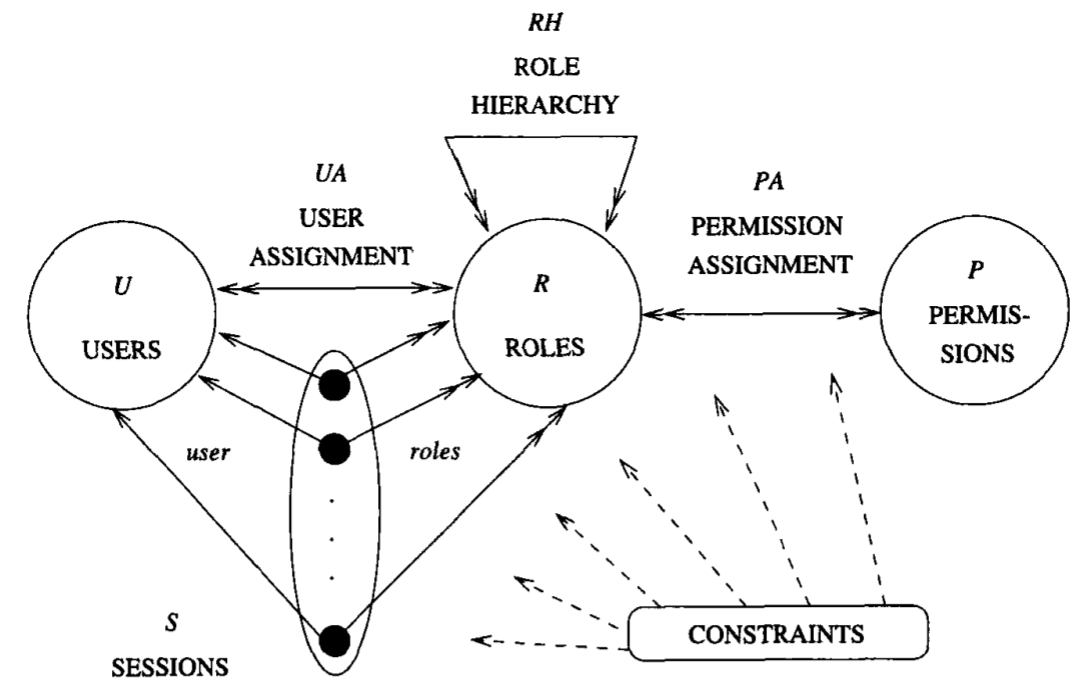
\includegraphics[width=\linewidth]{../figures/chapter2/Sandhu_notation.png}
	\caption{Graphical notation used by \cite{Sandhu96} to visualize $RBAC_3$}
	\label{fig:Sandhu_notation}
\end{figure}

\noindent
Unfortunatly \cite{Sandhu96} gives no details on how or why the notation is build up the way it is in his work.
Following graphical elements are used for this notation:

\begin{itemize}
\item A circle or ellipse represents a set ($U, R, P, S$).
\item A rounded rectangle represents a special set -- the set of constraints ($Constraints$).
\item A normal-headed unidirectional arrow represents a one-to-one assignment ($user$).
\item A double-headed unidirectional arrow represents a one-to-many assignment ($roles$).
\item A double-headed bidirectional arrow represents a many-to-many assignment relation ($UA, PA, RH$).
\item A normal-headed unidirectional dotted arrow represents a constraint.
Six arrows of this type are pointing symbolically from the set of constraints in the direction of all model components constraints can be potentially defined on.
\end{itemize}
%TODO: Better a table?

\noindent
A set has its name and its identifier in its center.
An arrow -- except the constraint arrow -- has its name and its identifier next to it.

Furthermore the \textit{Sessions} set ($S$) is not directly connected with arrows to other components.
It is drawn with large black dots inside, which represent single elements of this set.
These set elements are then connected to other components with certain arrows.
Three small black dots (in this case aligned horizontally) indicate that there are potentially more than just those three set elements (the number of sessions is not limited per definition).

This diagram is often used in a simplified form (for example in \citep{Amthor18}) that directly connects the \textit{Sessions} set -- like the other sets -- with just one arrow to \textit{Users} and one to \textit{Roles} and does not display single set elements of \textit{Sessions}.
Also worth mentioning is that $RH$ is drawn as a loop. 
It is pointing from \textit{Roles} ($R$) to \textit{Roles} with a double-headed bidirectional arrow.

%maybe my own gsl from bachelor thesis?


%\subsection{Security Model Core}
%\label{model_core}
%Over the years many different security models emerged for special purposes and requirements.
%They heavily vary and differ in their structure and design.
%Comparing them or even parts of them for analysis or evaluation purposes is not always possible per se.
%Methods to analyze a model concerning a given security property have to be adapted to every model they should run on.
%So \cite{Poelck14} proposed the Security Model Core to describe and formalize all possible security models in one meta model in a homogeneous way.

%\begin{xdefinition}[Security Model Core]
%\label{def:SecurityModelCore}
%The Security Model Core is a 5-tuple 
%$(Q, \Sigma , \delta , q_{0}, E)$ with 
%$Q$ as state space,
%$\Sigma$ as input alphabet, 
%$\delta: Q \times \Sigma \rightarrow Q$ as state transition function, 
%$q_0$ as initial state and 
%$E$ as static extension vector.
%\end{xdefinition}

%The definition of model components depends on the specialization of the corresponding model core and is done in six steps by identifying and defining those components.



\section{Aspect-oriented Security Engineering and Entity-Labeling Aspect}
\label{AOSEEL}
In this section the Aspect-oriented Security Engineering proposed by \citep{Amthor18} is described with focus on its Entity-Labeling aspect.
The content of this section will act as fundamental basis of information for designing a graphical specification language for the Entity-Labeling aspect later in chapter \ref{gsl_design}.


\subsection{Aspect-oriented Security Engineering}
\label{AOSE}
Aspect-oriented Security Engineering (AOSE) is a new approach proposed by \cite{Amthor18} to improve the process of model-based security engineering.
With an increasing number and complexity of security models the engineering process that goes along also became more complex and therefore prone to human errors.

\cite{Amthor18} claims to close semantic gaps between model engineering, model analysis and formal policy specification in the process of security engineering to reduce the potential impact of human errors.
These three steps and how they connect are depicted in figure \ref{fig:AOSE}.

\begin{figure}[htb]
	\centering
	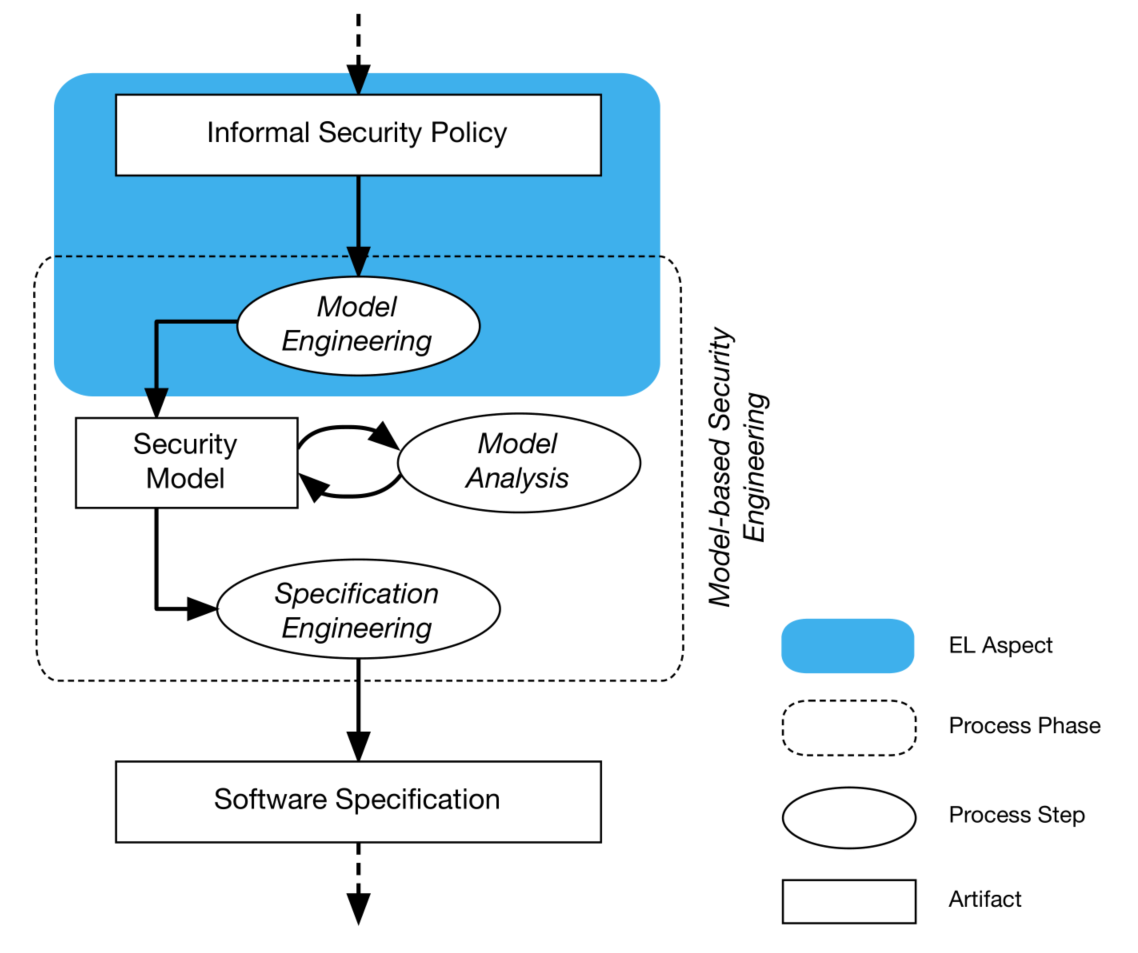
\includegraphics[scale=0.4]{../figures/chapter2/AOSE.png}
	\caption{Steps in the process of model-based security engineering \citep{Amthor18}}
	\label{fig:AOSE}
\end{figure}

\noindent
AOSE roughly adopts the idea of the aspect-oriented programming paradigm.
It tailors all steps to aspects, which are non-functional requirements of the engineering process like determining requirements of policy semantics or analyzing certain security goals.
There are two major classes \cite{Amthor18} proposes for aspects regarding AOSE: related to policy semantics and related to policy analysis.
One of several aspects proposed is Entity-Labeling.

According to \cite{Amthor18} an aspect-oriented security model is formally defined as:

\begin{xdefinition}[Aspect-oriented security model] 
A aspect oriented security model is defined as $\langle \mathcal{M},\mathcal{A},sem \rangle$ with:

\vspace{-2mm}
\begin{itemize}
\setlength\itemsep{0em}
\item $\mathcal{M}$ as finite set of model component identifiers
\item $\mathcal{A}$ as set of semantic category identifiers (aspect)
\item $sem : \mathcal{A} \rightarrow 2^\mathcal{M}$ as semantical application of $\mathcal{A}$ to $\mathcal{M}$
\end{itemize}
\end{xdefinition}



\subsection{Entity-Labeling Aspect}
\label{EL}
The Entity Labeling aspect (EL) is one possible aspect $\mathcal{A}$ in context of AOSE.
It is designed to formally specify policy semantics typically found in operating systems and middleware systems.
It bridges the gap between informal policy and formal model by supporting its transformation (see highlighted part in figure \ref{fig:AOSE}).
EL classifies model components into six semantic categories:


\begin{description}
\item[1) Entity Set (ES)]\hfill \\
A set of entity identifiers in the domain of an AC system.
\item[2) Label Set (LS)]\hfill \\
A set of legal label values.
\item[3) Label Assignment (LA)]\hfill \\
An association between entities and labels.
\item[4) Access Rule (AR)]\hfill \\
A logical rule that defines, based on a set of entity labels, which operations may be legally performed on entities corresponding to these labels. Model components in AR thus reflect a policy’s access control function (ACF).
\item[5) Relabeling Rule (RR)]\hfill \\
A logical rule for legal label changes.
\item[6) Model Constraint (MC)]\hfill \\
Constraints over model components that must be satisfied in every model state.
\end{description}

\noindent
According to these categories, we define the EL aspect as following:

\begin{xdefinition}[Entity-Labeling aspect] 
The entity labeling aspect of a security policy is defined as 
$\mathcal{A}_{EL} = \lbrace ES,LS,LA,AR,RR,MC\rbrace $
where $ES$, $LS$, $LA$, $AR$, $RR$, and $MC$ denote categories of model components defined as following:



\end{xdefinition}



\section{Graphical notation models}
\label{graphical_notations}

\subsection{Unified Modeling Language}
\label{UML}
The \textit{Unified Modeling Language} (UML) is a graphical modeling language to specify, visualize, design and document software \citep{UML_OMG}.
UML became a widely used tool in software development and was standardized by The Object Management Group in 1997 and also was approved as official ISO standard in 2005 \citep{UML_ISO}.

UML defines terms and relationships between those terms, as well as a graphical notation for those.
The current version of UML (2.5) contains 14 different types of diagrams.
Every diagram illustrates information according to one specific aspect.
UML diagrams are classified into static and dynamic types, but they can have fuzzy borders and mixed forms as well.
Static diagram types describe structural properties, dynamic diagram types behavioral properties.



\subsubsection{Components}
Components an UML diagram is build up with are classified into \textit{elements} and \textit{relationships}:

\begin{description}
\item[1) Elements]\hfill \\
Elements are the main objects in a UML diagram.
Graphically elements are based on closed shapes like boxes or ellipses.
They usually have a name or identifier in form of text in the center of their shape. Horizontal lines can be used to separate an element into two or more sections (see \textit{class diagram}). \\
Examples: Classes, components, nodes, objects, packages (see figure \ref{fig:UML_elements})

\begin{figure}[htb]
	\centering
	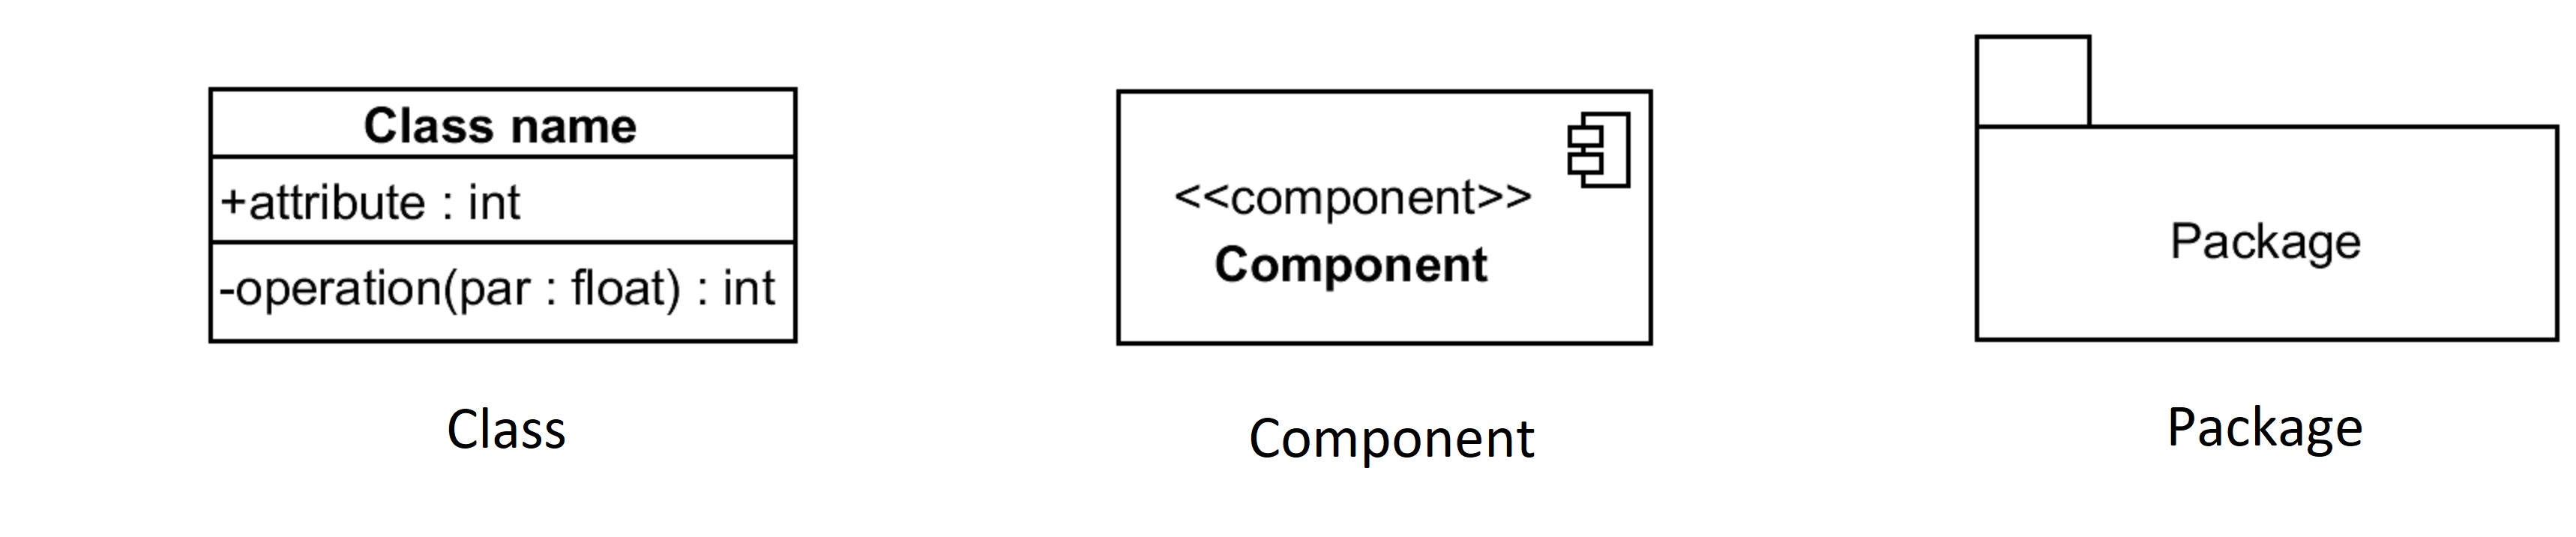
\includegraphics[scale=0.7]{../figures/chapter2/UML_elements.png}
	\caption{Selection of UML elements}
	\label{fig:UML_elements}
\end{figure}

\item[2) Relationships]\hfill \\
Relationships can connect two or more elements.
Graphically relationships are based on lines.
Optionally they can have a shape at one end to indicate some kind of direction.
They can vary in form by having differently drawn lines (solid, dotted), shaped arrows.
They can have several angles (preferable $90^{\circ}$ or $45^{\circ}$) to run on a clearly laid out path.
Lines do not collide if possible. \\
Examples: Dependency, association, generalization, include, extend (see figure \ref{fig:UML_relationships})

\begin{figure}[htb]
	\centering
	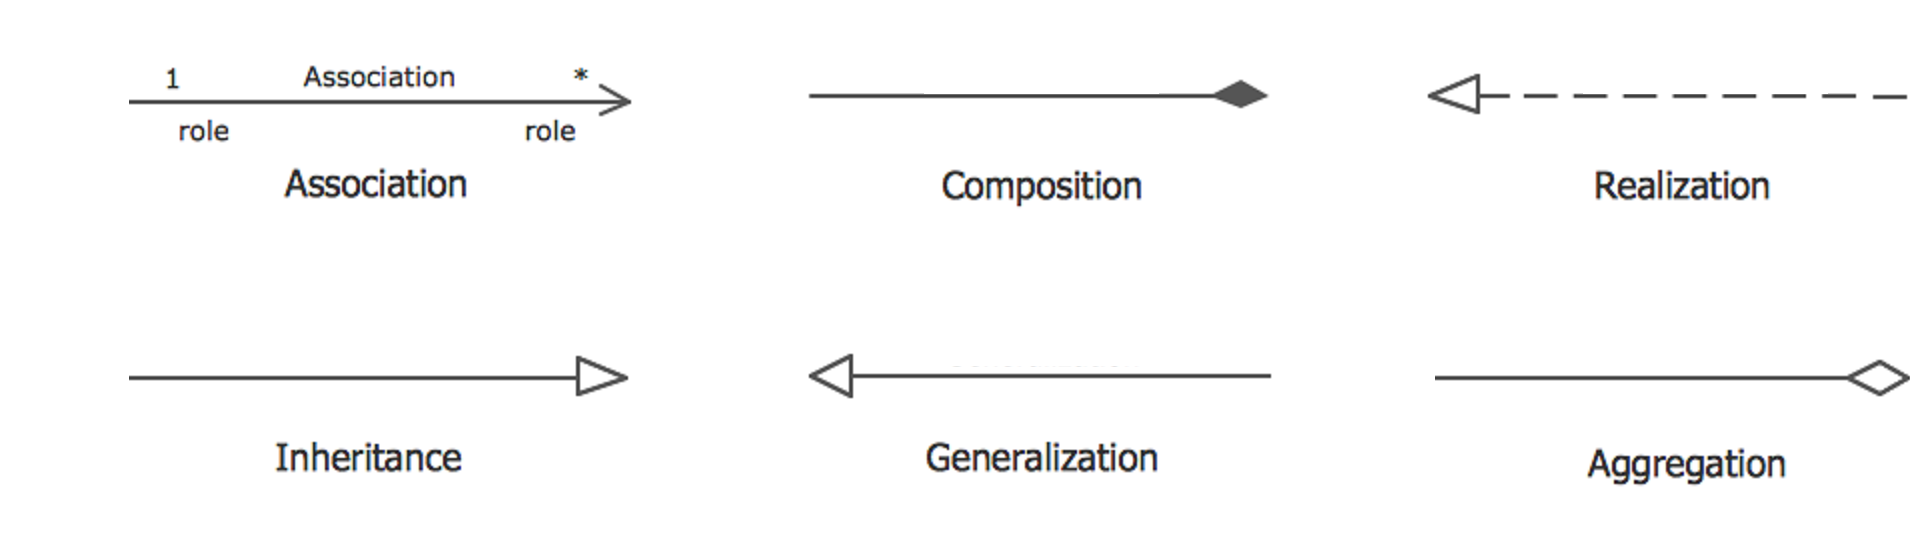
\includegraphics[scale=0.7]{../figures/chapter2/UML_relationships.png}
	\caption{Selection of UML relationships}
	\label{fig:UML_relationships}
\end{figure}
\end{description}

\noindent 
Class diagrams can have different levels of detail.
For example the class element has a simple symbolic form as well as an extended form with detailed information about its key words, attributes and operations (see figure \ref{fig:Class}).

\begin{figure}[htb]
	\centering
	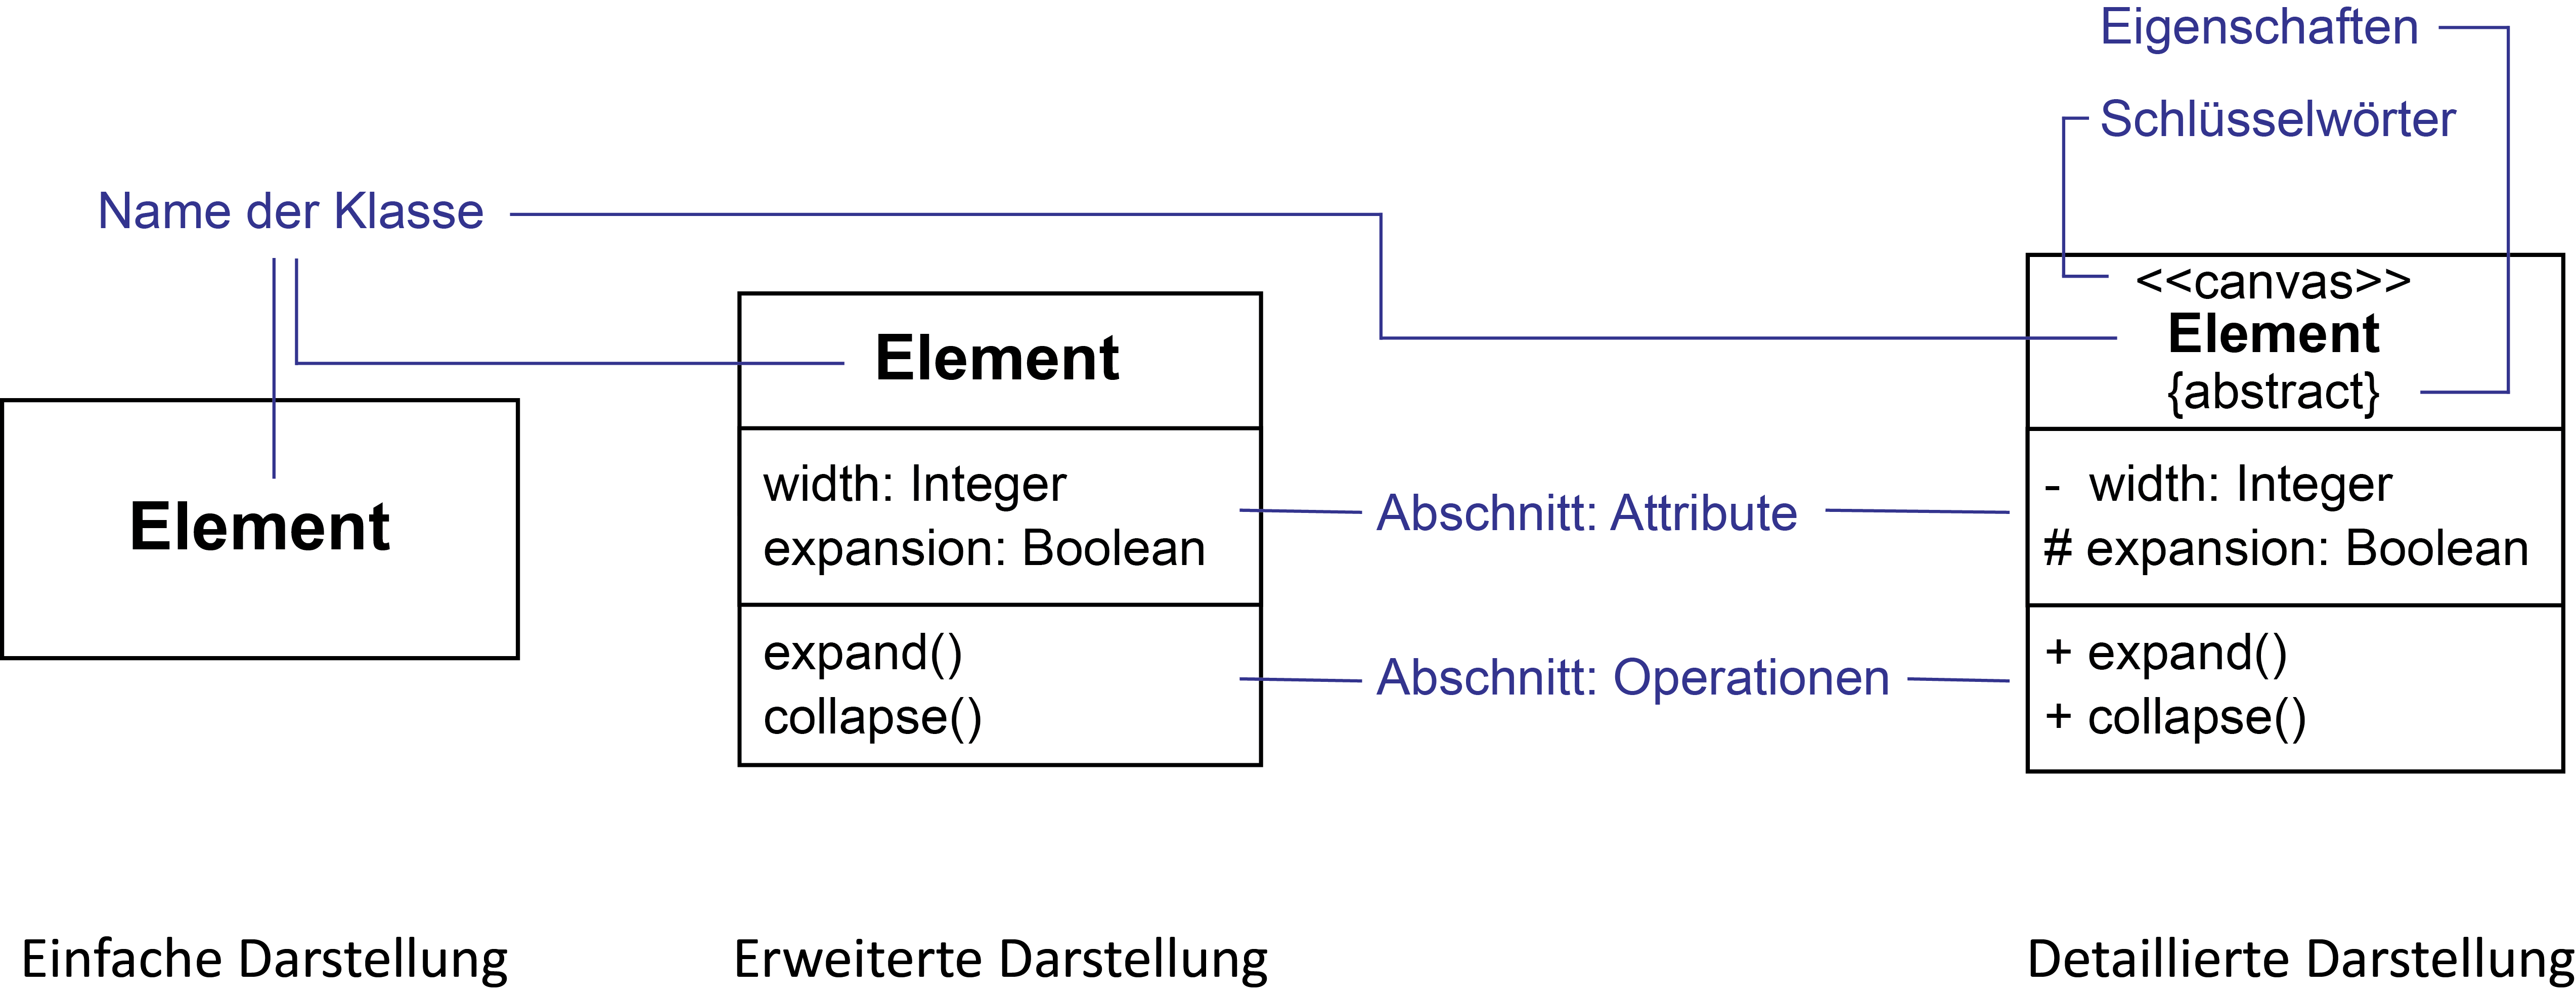
\includegraphics[scale=0.6]{../figures/chapter2/UML_Klassen2.png}
	\caption{Class diagrams with different level of detail}
	\label{fig:Class}
\end{figure}



\subsubsection{Additional annotations}
UML has symbols and textual identifiers to visualize certain properties.
A class diagram for example has the following symbols to indicate visibility of attributes and operations: + for \textit{public}, \# for \textit{protected} and - for \textit{private} (see figure \ref{fig:UML_class_diagram}).

%TODO: UML class diagram
%\begin{figure}[htb]
%	\centering
%	\includegraphics[scale=0.6]{../figures/chapter2/UML_class_diagram.png}
%	\caption{UML class diagram example with multiplicities}
%	\label{fig:UML_class_diagram}
%\end{figure}

\noindent 
With \textit{multiplicities} an element can be constrained regarding its number in context of an relationship.
The notation is placed at the connection point of class and relationship component.
The format for multiplicity bounds is defined by the UML specification 2.5 \citep{UML_OMG} in Backus-Naur form (BNF) as in listing \ref{BNF_multiplicity}.

\setlength{\grammarparsep}{10pt plus 1pt minus 1pt} % increase separation between rules
\setlength{\grammarindent}{13em} % increase separation between LHS/RHS 

\vspace{0.4cm}
\noindent
\begin{BNF}
\fbox{
\parbox[b]{\textwidth}{
\begin{grammar}
<multiplicity> ::= <multiplicity-range> [ [ `$\lbrace$' <order-designator> [ `,' <uniqueness-designator> ] `$\rbrace$' ] |
[ `$\lbrace$' <uniqueness-designator> [ `,' <order-designator> ] `$\rbrace$' ] ]

<multiplicity-range> ::= [ <lower> `..' ] <upper>

<lower> ::= <value-specification>

<upper> ::= <value-specification>

<order-designator> ::= `ordered' | `unordered'

<uniqueness-designator> ::= `unique' | `nonunique'
\end{grammar}
}
}
\caption{UML multiplicity syntax in BNF}
\label{BNF_multiplicity}
\end{BNF}
\vspace{0.3cm}

\noindent
For the sake of convenience we assume the literal <value-specification> being an integer number (0 or 1 in most cases) or * to indicate the end of a boundless interval.

Furthermore it is worth mentioning that UML does not use any color for its diagrams.
This makes it compatible, easy and fast for hand-drawing.
Coloring always remains a not officially specified option to highlight certain parts of a diagram, e.g. to set a focus for an accompanying text.


\subsection{Entity-Relationship model}
\label{ER}
The entity-relationship model (ER) is a model to describe classified objects (entities) and how they are interrelated.
It was developed to illustrate information in databases on a conceptual level and became a popular tool for requirement analysis in this domain.
In contrast to UML (see section \ref{UML}), which is a collection of multiple diagram types, ER only has one type of diagram: The Entity-Relationship diagram (ERD).

Also unlike UML ER is not an officially specified standard.
Furthermore ER has some slightly different notation variants (Chen, Bachman, etc.), which will be discussed in section \ref{ERD_notations}.
The figures in this subsection are in Chen notation.
Figure \ref{fig:ERD_minimal_example} shows an example of an ERD.


\begin{figure}[htb]
	\centering
	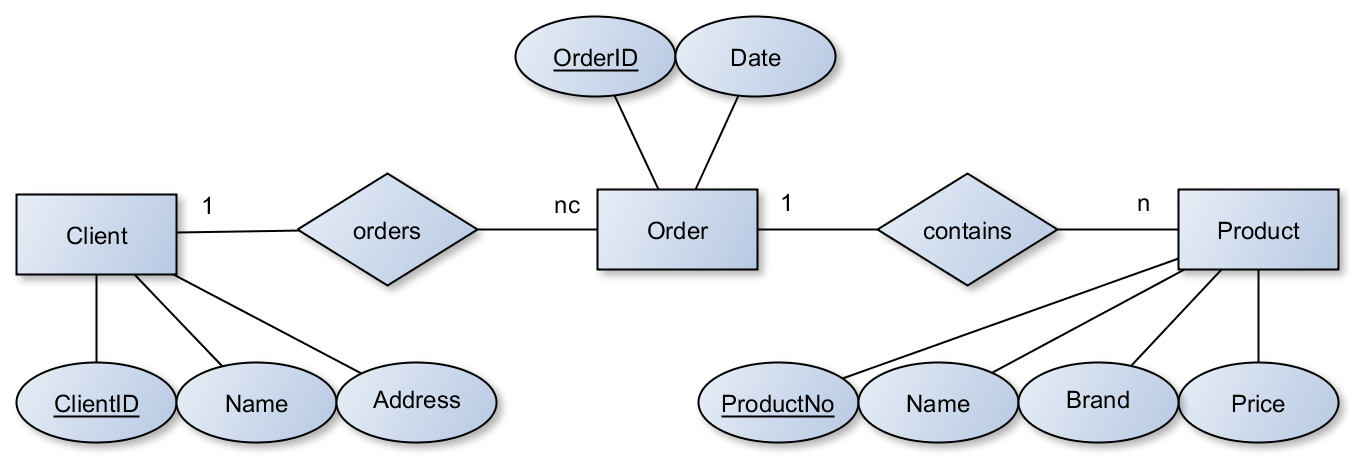
\includegraphics[width=\linewidth]{../figures/chapter2/ERD_minimal_example.png}
	\caption{ERD example}
	\label{fig:ERD_minimal_example}
\end{figure}

\subsubsection{Components}
ERDs are build up with the following components \citep{Kleuker11}:

\begin{description}
\item[1) Entity type]\hfill \\
The most important artifact of ER is probably the entity.
It represents an individual and unambiguously identifiable object.
An entity is characterized by its properties.
An \textit{entity type} is a template for entities that summarizes all their attributes.
Entities can be interpreted as instances of an entity type with concrete values.
Graphically an entity type is a simple rectangle with its name in its center.

\begin{figure}[htb]
	\centering
	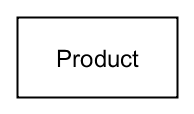
\includegraphics[scale=0.4]{../figures/chapter2/ERD_entity.png}
	\caption{Entity object of an ERD}
	\label{fig:ERD_entity}
\end{figure}

\item[2) Relationships]\hfill \\
Relationships can connect two or more entities and describe how they are interrelated.
In contrast to UML (see \ref{UML}) relationship is not represented with a simple lines, but with a rhombus with the relationship name in its center.
This rhombus is then connected to two or more entities with simple lines.
These lines may have symbols at their end to indicate properties of the connected entities in context of the relationship.

\begin{figure}[htb]
	\centering
	
\includegraphics[scale=0.4]{../figures/chapter2/ERD_relationship.png}
	\caption{Relationship object of an ERD}
	\label{fig:ERD_relationship}
\end{figure}

\item[3) Attributes]\hfill \\
Attributes are properties of entites or relationships.
Graphically an attribute is a single ellipse with its name in its center.
It is connected to an entity or to a relationship with the help of a simple line.

\begin{figure}[htb]
	\centering
	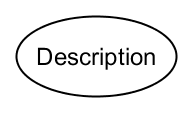
\includegraphics[scale=0.4]{../figures/chapter2/ERD_attribute.png}
	\caption{Attribute object of an ERD}
	\label{fig:ERD_}
\end{figure}
\end{description}

\subsubsection{Additional annotations}
To specify the amount of entities in context of a relationship the following indicators for \textit{cardinalities} are used:

\begin{itemize}
\setlength\itemsep{0em}
\item \textbf{1} to indicate a relationship to exactly one entity.
\item \textbf{c} to indicate a relationship to no or one entities.
\item \textbf{n} to indicate a relationship to one or multiple entities.
\item \textbf{nc} to indicate a relationship to no, one or multiple entities.
\end{itemize}

\noindent
Cardinalities can be upper case (N) or lower case (n) with no semantic difference.
A relationship can be read in two directions.
For example the \textit{orders}-relationship in figure \ref{fig:ERD_minimal_example}:

\begin{itemize}
\setlength\itemsep{0em}
\item An order is connected to exactly one client (left-to-right).
\item A client is connceted to no, one or multiple orders (right-to-left).
\end{itemize}

\noindent
An entity type needs to have a \textit{primary key} defined in order to have its elements unambiguously identifiable.
The primary key is an attribute or a combination of attributes of the entity type and has to be unique among all other attribute values.
A primary key attribute is graphically indicated with an underlined name (see \textit{ClientID} in figure \ref{fig:ERD_minimal_example}).

Besides this basic system, ERDs can indicate some additional information.
For example besides those elements described above, there are variants of them with a double frame line to indicate a \textit{weak} property (no primary key, therefore dependent to parent elements) or a dashed frame line to indicate a \textit{multivalued} property.
In context of this work those will not be relevant.

%UML
Notable is that an ER model can be visualized with the help of UML to some degree.
When entity types are treated as classes, entities as objects, relationships as associations, attributes as instance variables and cardinalities as multiplicities an UML \textit{class diagram} can be used to build up a diagram similar to an ERD.

\begin{figure}[htb]
	\centering
	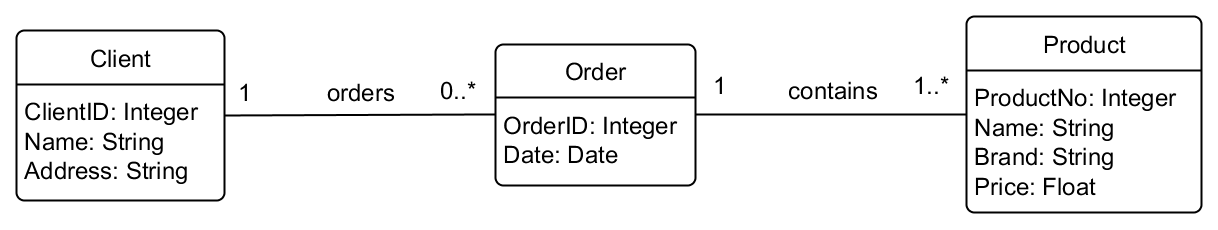
\includegraphics[width=\linewidth]{../figures/chapter2/ERD_as_UML.png}
	\caption{Information from figure \ref{fig:ERD_minimal_example} modeled as UML class diagram}
	\label{fig:ERD_as_UML}
\end{figure}

As seen in figure \ref{fig:ERD_as_UML} the diagram differs from the diagram in figure \ref{fig:ERD_minimal_example} in almost all aspects, but still they are easy to read and to translate into each other.

%The data modeling technique can be used to describe any ontology (i.e. an overview and classifications of used terms and their relationships) for a certain area of interest


\subsubsection{Notations}
\label{ERD_notations}
As already mentioned ER is not standardized and has different notation variants.
The notation variants only differ in their symbol usage at the end of lines.
Here is a short overview on how some of these differ in their appearance:

\begin{figure}[htb]
	\centering
	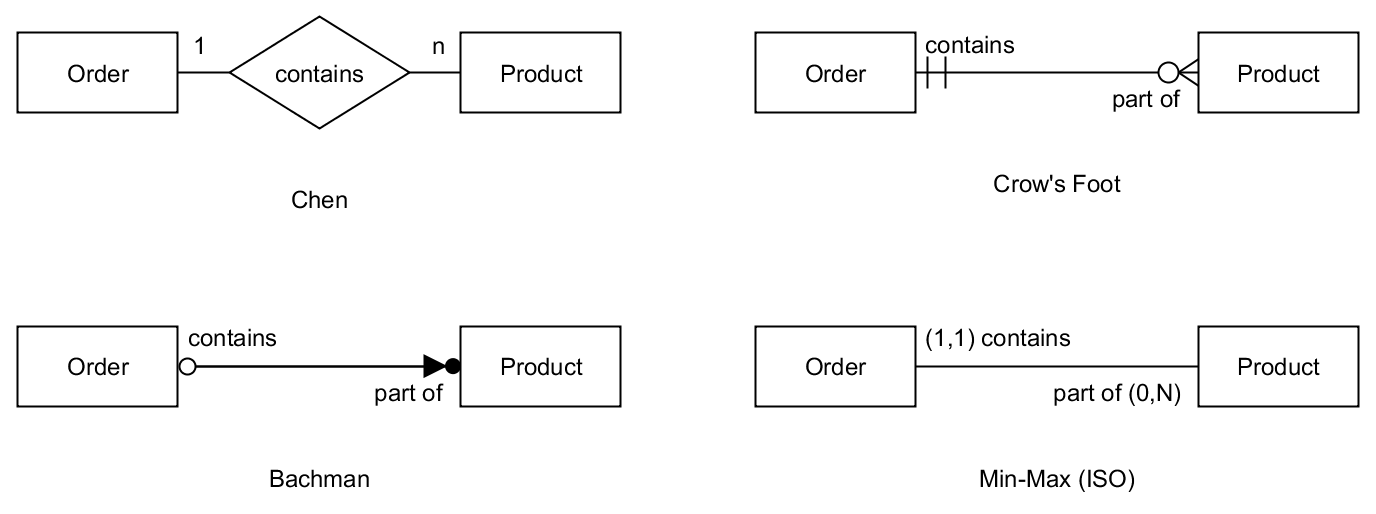
\includegraphics[scale=0.5]{../figures/chapter2/ERD_notations.png}
	\caption{Simple example in different ER notation variants}
	\label{fig:ERD_notations}
\end{figure}




\section{Gestalt laws and human optical perception}
\label{gestalt_laws_and_human_optical_perception}


\subsection{Gestalt laws}
\label{gestalt_laws}


\subsection{Human optical perception}
\label{human_optical_perception}




\section{GUI Design}
\label{gui_design}


\subsection{Design Patterns}
\label{design_patterns}


\subsection{Usability}
\label{usability}




\cleardoublepage
\chapter{Design: Graphical specification language}
\label{gsl_design}


\section{Concept}
\label{gsl_concept}
approach, basic ideas, adoptions from literature

\section{Elements}
\label{gsl_elements}


\section{Relationships}
\label{gsl_relationships}


\section{Structure}
\label{gsl_structure}


\section{Visualization on the higher abstraction level}
\label{higher_abstraction_level}




\cleardoublepage
\chapter{Design: Editor GUI}
\label{editor_design}


\section{Structure}
\label{editor_structure}


\section{Sections}
\label{editor_sections}




\cleardoublepage
\chapter{Implementation}
\label{implementation}
	
	
\section{Implementation base}
\label{implementation_base}
Qt, MVC

\section{Structure}
\label{implementation_structure}
	
	
\section{GUI sections}
\label{implementation_sections}




\cleardoublepage
\chapter{Evaluation}
\label{evaluation}


\section{Graphical specification language}
\label{evaluation_gsl}


\section{Editor}
\label{evaluation_editor}


\cleardoublepage
\chapter{Conclusion}
\label{conclusion}
\blindtext



\cleardoublepage
\chapter{Summary}
\label{summary}
\blindtext



% Anhang
%\cleardoublepage
%\tocentry{Anhang}
%\renewcommand{\thesection}{\Alph{section}}
%\markboth{Anhang}{}
%\chapter*{Anhang}
%\section{Kapitel 1}
%\section{Kapitel 2}
%\label{appendix}




% Literaturverzeichnis
\cleardoublepage
\DeclareRobustCommand{\citeext}[1]{\citeauthor{#1}~\cite{#1}}
\bibliographystyle{plainnat}

\bibliography{other/db}

\tocentry{Bibliography}





\end{document}